%% This is file `elsarticle-template-1-num.tex',
%%
%% Copyright 2009 Elsevier Ltd
%%
%% This file is part of the 'Elsarticle Bundle'.
%% ---------------------------------------------
%%
%% It may be distributed under the conditions of the LaTeX Project Public
%% License, either version 1.2 of this license or (at your option) any
%% later version.  The latest version of this license is in
%%    http://www.latex-project.org/lppl.txt
%% and version 1.2 or later is part of all distributions of LaTeX
%% version 1999/12/01 or later.
%%
%% Template article for Elsevier's document class `elsarticle'
%% with numbered style bibliographic references
%%
%% $Id: elsarticle-template-1-num.tex 149 2009-10-08 05:01:15Z rishi $
%% $URL: http://lenova.river-valley.com/svn/elsbst/trunk/elsarticle-template-1-num.tex $
%%
\documentclass[preprint,12pt]{elsarticle}

%% Use the option review to obtain double line spacing
%% \documentclass[preprint,review,12pt]{elsarticle}

%% Use the options 1p,twocolumn; 3p; 3p,twocolumn; 5p; or 5p,twocolumn
%% for a journal layout:
%% \documentclass[final,1p,times]{elsarticle}
%% \documentclass[final,1p,times,twocolumn]{elsarticle}
%% \documentclass[final,3p,times]{elsarticle}
%% \documentclass[final,3p,times,twocolumn]{elsarticle}
%% \documentclass[final,5p,times]{elsarticle}
%% \documentclass[final,5p,times,twocolumn]{elsarticle}

%% The graphicx package provides the includegraphics command.
\usepackage{graphicx}
%% The amssymb package provides various useful mathematical symbols
\usepackage{amssymb}
%% The amsthm package provides extended theorem environments
%% \usepackage{amsthm}

%% The lineno packages adds line numbers. Start line numbering with
%% \begin{linenumbers}, end it with \end{linenumbers}. Or switch it on
%% for the whole article with \linenumbers after \end{frontmatter}.
\usepackage{lineno}

\usepackage{hyperref}

\usepackage{caption}
\usepackage{subcaption}

%% natbib.sty is loaded by default. However, natbib options can be
%% provided with \biboptions{...} command. Following options are
%% valid:

%%   round  -  round parentheses are used (default)
%%   square -  square brackets are used   [option]
%%   curly  -  curly braces are used      {option}
%%   angle  -  angle brackets are used    <option>
%%   semicolon  -  multiple citations separated by semi-colon
%%   colon  - same as semicolon, an earlier confusion
%%   comma  -  separated by comma
%%   numbers-  selects numerical citations
%%   super  -  numerical citations as superscripts
%%   sort   -  sorts multiple citations according to order in ref. list
%%   sort&compress   -  like sort, but also compresses numerical citations
%%   compress - compresses without sorting
%%
%% \biboptions{comma,round}

% \biboptions{}

\journal{Journal Name}

\begin{document}

\begin{frontmatter}

    %% Title, authors and addresses

    \title{2D Seismic Data Classification using Convolutional Neural Network and 2D Synthetic Data}

    %% use the tnoteref command within \title for footnotes;
    %% use the tnotetext command for the associated footnote;
    %% use the fnref command within \author or \address for footnotes;
    %% use the fntext command for the associated footnote;
    %% use the corref command within \author for corresponding author footnotes;
    %% use the cortext command for the associated footnote;
    %% use the ead command for the email address,
    %% and the form \ead[url] for the home page:
    %%
    %% \title{Title\tnoteref{label1}}
    %% \tnotetext[label1]{}
    %% \author{Name\corref{cor1}\fnref{label2}}
    %% \ead{email address}
    %% \ead[url]{home page}
    %% \fntext[label2]{}
    %% \cortext[cor1]{}
    %% \address{Address\fnref{label3}}
    %% \fntext[label3]{}


    %% use optional labels to link authors explicitly to addresses:
    %% \author[label1,label2]{<author name>}
    %% \address[label1]{<address>}
    %% \address[label2]{<address>}

    \author[label1]{Alice Y. Yang}
    \author[label2]{Musa Manzi}
    \author[label2]{Michael Westgate}
    \author[label2]{Ling Cheng}

    \address[label1]{Cape Town, South Africa}
    \address[label2]{Johannesburg, South Africa}

    \begin{abstract}
        %% Text of abstract
        The following paper looks at classifying 2-dimensional seismic data extracted
        from South African geo-location using a Convolutional Neural Network (CNN)
        that is trained with synthetic data. The purpose of this paper illustrates the
        difficulties in working with seismic data and the precision needed for automating
        feature extraction within the CNN architecture in order to achieve
        a 90\%. The CNN architecture is mainly constructed using 2D convolutional
        and max-pooling layers.
    \end{abstract}

    \begin{keyword}
        2D Seismic Data \sep Convolutional Neural Network \sep Synthetic Data \sep Gold mines
        %% keywords here, in the form: keyword \sep keyword

        %% MSC codes here, in the form: \MSC code \sep code
        %% or \MSC[2008] code \sep code (2000 is the default)

    \end{keyword}

\end{frontmatter}

%%
%% Start line numbering here if you want
%%
\linenumbers

%% main text
\section{Introduction}
In recent years, Artificial Intelligence (AI) has grown exponentially
and has been applied to multiple disciplines. It is no surprise that it has
found its way into geology. Given that the geologist work with large sets of
geological data to map both surfaces of the earth and faults below the surface,
which has an enormous potential for AI. The traditional method of interpreting
subsurface data includes manual fault picking and horizons on section, which is
then followed by qualitative enhancements \cite{seismic_interpretation}. The qualitative
enhancement techniques involves structurally-oriented semblance, tensor, duo and etc.
for highlighting the fault structure within the subsurface seismic dataset \cite{seismic_interpretation}.
This paper addresses alternative approaches for classifying seismic data using Artificial
Intelligence and more specifically, Convolutional Neural Network (CNN) for classifying
2D seismic image data. The objective of the purposed technique is to detect whether
intersecting faults or non-intersecting faults are present within 2D seismic data.
The paper is structured such that Section \ref{sec:background} provides a brief background
of the techniques used in this paper. Section \ref{sec:methodology} describes the methodology
and the process of achieving the results addressed in Section \ref{sec:results}, before concluding
in Section \ref{sec:conclusion}.

\section{Background}
\label{sec:background}

\subsection{Convolutional Neural Network}
The Convolutional Neural Network (CNN) is a subsidiary of supervised23
technique within in the deep learning field. It is commonly employed for24
image classification purposes due to its exceptional ability to purpose image25
analysis using the mathematical convolutional operation and obtaining high26
classification accuracies \cite{krizhevsky2012imagenet, zhiqiang2017review}.
Due to the CNN’s high classification accuracy, it has been utilized within
multiple fields including the geological realm for earthquake detection and
location \cite{perol2018convolutional}, seismic inversions \cite{das2019convolutional},
and fault detection \cite{wu2019faultseg3d, xiong2018seismic}.

Given that the CNN is a supervised neural network, it learns images features
based in order to form an end-to-end model with the trained parameters
through the gradient descent method. Therefore, the CNN model makes use
of connected weights within the network as a form of sharing “knowledge”
and reducing the number of training parameters, and as a result also reducing
redundant complexity \cite{zhiqiang2017review, chumerin2017convolutional}.
In general, the first few layers of the CNN architecture
consists of convolution and pooling layers, whilst the layers following
there after are fully-connected network \cite{wu2019faultseg3d, lecun1998gradient}.

The training of the CNN is conducted mainly using both back- and forward
propagation algorithms to adjust the weights of the neurons based on
the given training data. The objective of the back-propagation algorithm is
to adjust the weights to minimise loss based on the network’s overall outcome
and the target. The network’s overall outcome is obtained using the forward
propagation. The back-propagation loss function, $E(W,b)$ is expressed in
\ref{eq:mean_squared_error} as the Mean Squared Error (MSE).

\begin{equation}
    \label{eq:mean_squared_error}
    E(W, b) = \frac{1}{|Y|} \sum_{i=1}^{|Y|} (Y(i) - \bar{Y}(i)^{2})
\end{equation}

where $W$ is the weight value and $b$ is the bias value. Both the weight value,
$W$ and bias value, $b$ are updated during the back-propagation training according to
\ref{eq:weight_equation} and \ref{eq:bias_equation}, respectively.

\begin{equation}
    \label{eq:weight_equation}
    W_i = W_i - \eta \frac{\partial E(W,b)}{\partial W_i}
\end{equation}

\begin{equation}
    \label{eq:bias_equation}
    b_i = b_i - \eta\frac{\partial E(W,b)}{\partial b_i}
\end{equation}

where $\eta$ is the learning rate.

\section{Literature Review}
Wu, X. et al.performed image-to-image binary fault detection using a
fully-supervised CNN \cite{wu2019faultseg3d}. The authors made use of 3D seismic images which
where labelled with ones for fault and zeros elsewhere. The CNN model was
trained with 200 3D synthetic seismic images with a $128\times128\times128$ dimension
for each fault and non-fault category. The training of the neural network was
performed on a TITAN Xp GPU which took the authors approximately 2
hours to train. The authors validated the network with 20 pairs of unseen
synthetic image data, in which the network achieved a 95\% classification
accuracy. The generated synthetic data consists of faults at varying angles,
specially at $90^{\circ}$, $180^{\circ}$, and $270^{\circ}$. Additionally, the authors
applied the trained CNN to detect faults on surveyed 3D data from four different locations,
namely the Netherlands off-shore data, Clyde Petroleum Plc., Costa Rica
margin North West of Osa Peninsula, and Campos Basin which is off-shore
of Brazil.

Zheng, Y. et al. presents two separate case studies involving supervised
deep learning as an alternative for the conventional techniques in seismic
data interpretation and inversion \cite{zheng2019applications}. In the first case study, the authors
apply the CNN for seismic image classification as a way of interpretation.
The CNN is trained with 3D seismic volumes, such that images are classified
into two categories, namely, fault and non-fault. The fault data consists
of certain dips as well as azimuth, which are distinguishing features in the
data considered as faults. In the second case study, the authors present an
elastic model building, in which a CNN is trained to perform predictions
of 1D velocity and density profiles within the given seismic data. In both
case studies, the authors have trained the CNN models using synthetic data
and tested the models on survey field data. The authors have found that
both CNN models obtained effective and efficient predictions when testing
on field data, therefore showing high-quality fault picks. However, challenges
are presented when the authors worked with pre-stacked seismic inversions,
where subsurface geological variations and preconditioning of the input seismic
data plays an important factor in the ability of the CNN models to
perform accurate predictions.

The author, Zhao, T. presents an encoder-decoder CNN model for seismic
facies classification \cite{zhao2018seismic}. The architecture of the encoder-decoder CNN model
consists of an encoding component, in which the input data given to the
model is reduced and a decoding component, whereby the reduced data is
then expanded once again. The purpose of the encoding component is to
reduce the input data such that only the significant portions of the input data
is kept, whilst the decoding component further highlights and expands on the
significant data such that contributing noise within the input data is removed.
This allows for enhanced fault predictions in seismic faces. Additionally, the
author has compared the presented CNN model to the architecture of the
more traditional patch-base CNN model, in which the author found that the
patch-base CNN model requires less training effort compared to the encoder-
decoder CNN model, however the patch-based CNN produced suboptimal
predictions compared to the encoder-decoder CNN.

Di, H et al. introduces a CNN model for the application of salt-body
delineation from 3D seismic data \cite{di2018deep}. The authors have found the implementation
of the CNN model is far more superior when compared to the traditional
schemes of sample-based multi-attribute classification. The implemented
CNN model takes the local seismic patterns which are distinguishing
features within the target salt-body. Furthermore the CNN allows for optimal
mapping relationship between the seismic signals and the salt-bodies,
and as a result it does not require laborious manual attribute selection as
performed in the traditional classification schemes. The CNN model was
trained using synthetic data from the SEG-SEAM dataset.

Xiong, W. et al. developed a method which employs the CNN to automate
and map fault detection in 3D seismic images to mimic the traditional
approach by interpretors. The CNN is trained with image cubes obtained
from field data which are labelled as either fault or non-fault. The trained
CNN is then applied to unseen field data to predict the fault probabilities at
every location with given cube images. The authors have been able to obtain
a 99\% classification accuracy using the trained CNN.

\section{Methodology}
\label{sec:methodology}
The technique consists of two distinct processes. The first is training the
and the second is applying the trained CNN to unseen 2D seismic data. The seismic
data is extracted from South African geological sub-surfaces. The two processes are
illustrated in Figure \ref{fig:system_processes}, in which the training process is depicted on the left and
the test process on the right.

\begin{figure}[h]
    \centering
    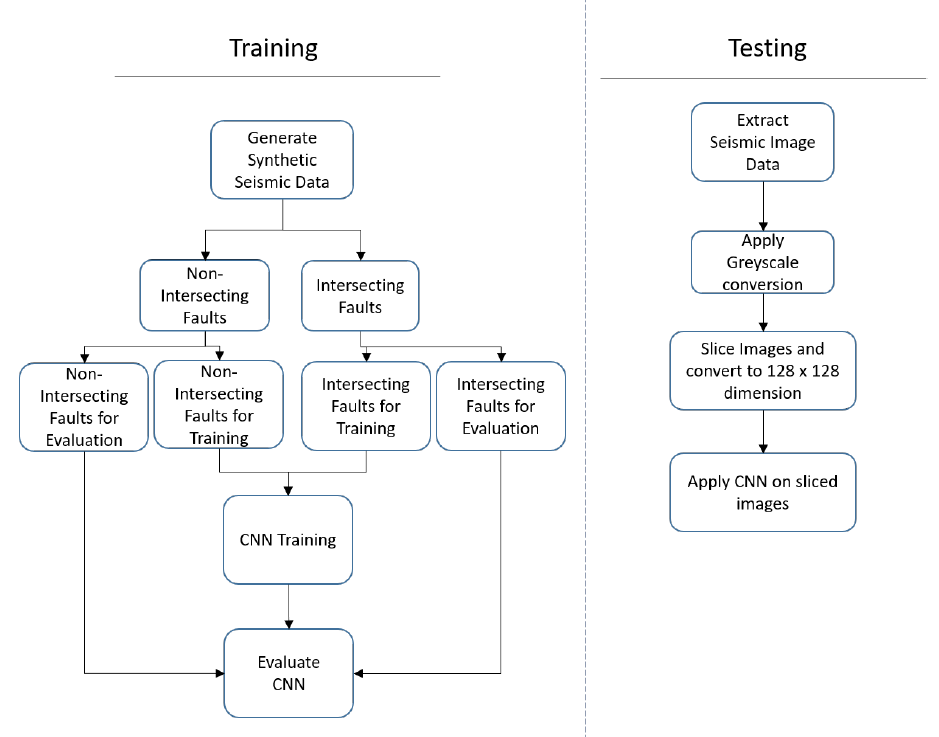
\includegraphics[scale=0.7]{images/system_processes.png}
    \caption{Diagrams illustrating the training and testing processes involving the
        Convolutional Neural Network.}
    \label{fig:system_processes}
\end{figure}

\subsection{Training Images}
The data used for training the CNN is taken from
\href{https://github.com/xinwucwp/faultSeg}{FaultSeg3D: using synthetic datasets to
    train an end-to-end convolutional neural network for 3D seismic fault segmentation}
whereby the data is given as three-dimensional $128 \times 128 \times 128$
seismic data, which is generated by Wu, X. et al \cite{wu2019faultseg3d}. The data is transformed
from 3D to 2D, by taking slices of the 3D block to generate 2D $128 \times 128$
seismic data. From the synthetic data, only the seismic data which has
intersecting and none-intersecting fault are selected. Figures in  \ref{subfig:intersecting_faults}
and \ref{subfig:highlighted_faults} illustrates the training data.
Both images \ref{subfig:non_intersecting_faults} and \ref{sub@subfig:highlighted_non_faults} are not used as part
of the training data, however are used to assist in the labelling of intersecting
and non-intersecting fault data. A total of 350 seismic images are used in
each category for the training of the CNN.

\begin{figure}
    \centering
    \begin{subfigure}[b]{.3\textwidth}
        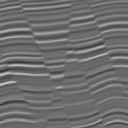
\includegraphics[width=\textwidth]{images/seismic_intersecting_fault.png}
        \caption{Seismic image with intersecting faults}
        \label{subfig:intersecting_faults}
    \end{subfigure}
    \begin{subfigure}[b]{.3\textwidth}
        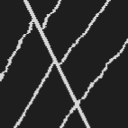
\includegraphics[width=\textwidth]{images/highlighted_interesecting_fault.png}
        \caption{Highlighted image with intersecting faults}
        \label{subfig:highlighted_faults}
    \end{subfigure}
\end{figure}

\begin{figure}
    \centering
    \begin{subfigure}[b]{.3\textwidth}
        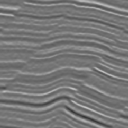
\includegraphics[width=\textwidth]{images/seismic_non_intersecting.png}
        \caption{Seismic image with non-intersecting faults}
        \label{subfig:non_intersecting_faults}
    \end{subfigure}
    \begin{subfigure}[b]{.3\textwidth}
        
\includegraphics[width=\textwidth]{images/highlighted_non_intersecting.png}
        \caption{Highlighted image with non-intersecting faults}
        \label{subfig:highlighted_non_faults}
    \end{subfigure}
\end{figure}

\subsection{Convolutional Neural Network}
The CNN is comprised of three distinct layers excluding the input and
output layer, namely 2D convolutional, max pooling and fully connected
layers. There are a total of four hidden layers in the neural network
architecture. The 2D convolutional layer makes use of the Rectified Linear
Unit (Relu) function. Figure \ref{fig:cnn_architecture} shows the detailed architecture of CNN. The
CNN is trained with 25 epochs. Figure \ref{fig:evaluation_model} shows the accuracy and validation
accuracy of the CNN at each epoch.

\begin{figure}
    \centering
    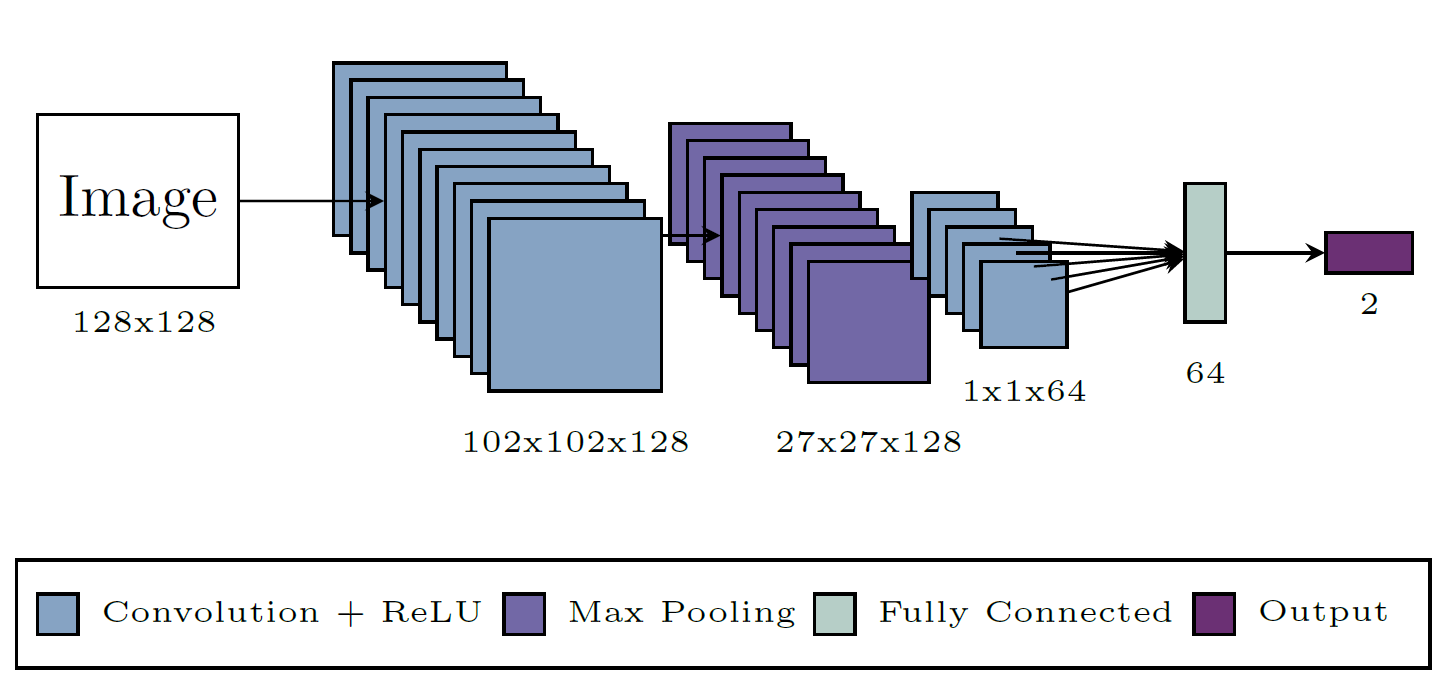
\includegraphics[width=\textwidth]{images/CNN_architecture.png}
    \caption{Figure illustrating the architecture of the Convolutional Neural Network}
    \label{fig:cnn_architecture}
\end{figure}

\begin{figure}
    \centering
    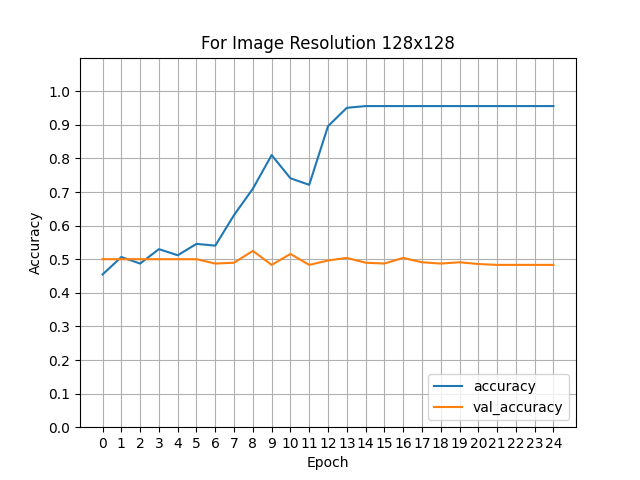
\includegraphics[width=\textwidth]{images/evaluate_model.png}
    \caption{Figure illustrating accuracy of the CNN at each epoch}
    \label{fig:evaluation_model}
\end{figure}


\subsection{Seismic Data Testing}
The seismic testing data consists of surface and edge detected images
of the orebody. The two image considered are shown in
Figure \ref{fig:orebody_surface_earth} and \ref{fig:highlighted_gold_mine},
in which both images are taken from South African gold mines.

\begin{figure}
    \centering
    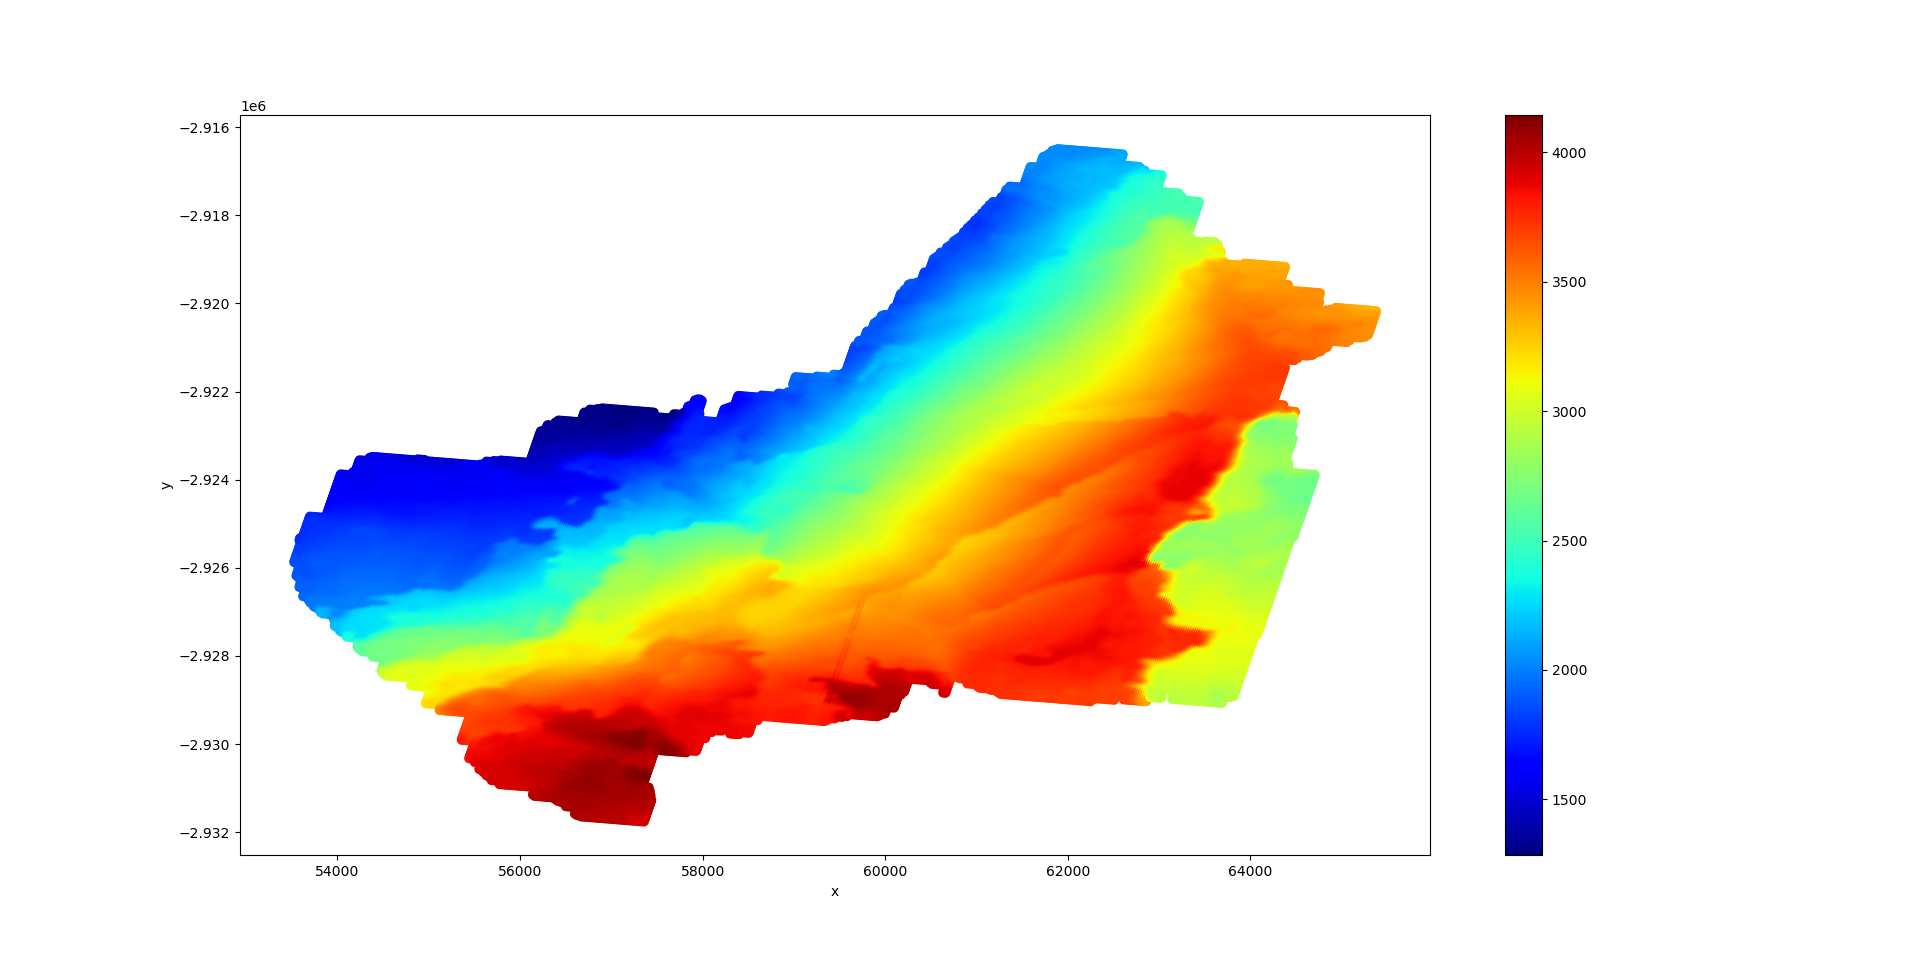
\includegraphics[width=\textwidth]{images/Orebody-surface_EarthVision_Gri.png}
    \caption{Figure illustrating the orebody surface extracted from a gold mine}
    \label{fig:orebody_surface_earth}
\end{figure}

\begin{figure}
    \centering
    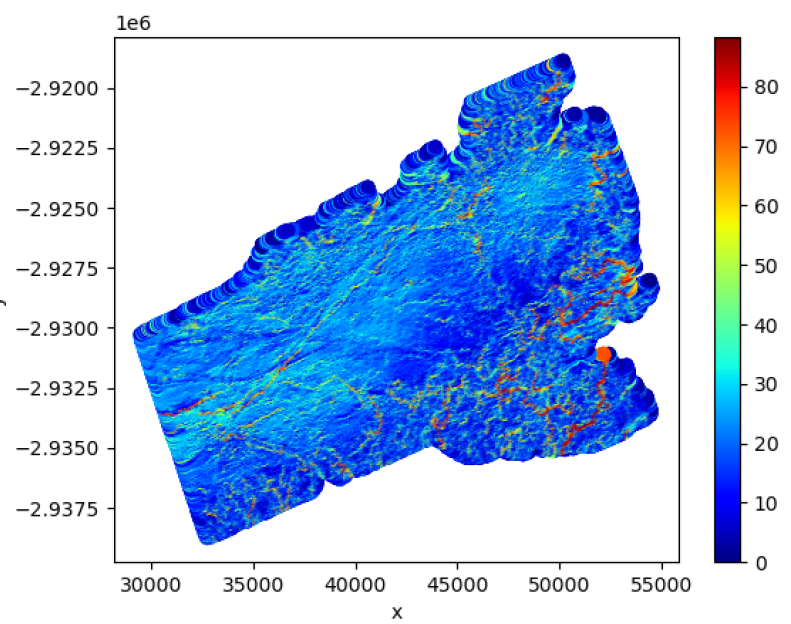
\includegraphics[width=\textwidth]{images/highlighted_orebody.png}
    \caption{Figure illustrating the orebody surface with highlighted edges extracted
        from the gold mine}
    \label{fig:highlighted_gold_mine}
\end{figure}

\section{Results}
\label{sec:results}

\section{Application}

\section{Conclusion}
\label{sec:conclusion}

%% The Appendices part is started with the command \appendix;
%% appendix sections are then done as normal sections
%% \appendix

%% \section{}
%% \label{}

%% References
%%
%% Following citation commands can be used in the body text:
%% Usage of \cite is as follows:
%%   \cite{key}          ==>>  [#]
%%   \cite[chap. 2]{key} ==>>  [#, chap. 2]
%%   \citet{key}         ==>>  Author [#]

%% References with bibTeX database:

% \bibliographystyle{model1-num-names}

%% New version of the num-names style
\bibliographystyle{elsarticle-num-names}
\bibliography{ref.bib}

%% Authors are advised to submit their bibtex database files. They are
%% requested to list a bibtex style file in the manuscript if they do
%% not want to use model1-num-names.bst.

%% References without bibTeX database:

% \begin{thebibliography}{00}

%% \bibitem must have the following form:
%%   \bibitem{key}...
%%

% \bibitem{}

% \end{thebibliography}


\end{document}

%%
%% End of file `elsarticle-template-1-num.tex'.